	\section{ کدزنی و پیاده سازی‬}
	
	\subsection{بخش‌های ۱ تا ۴}
	
	\subsubsection{مقدمه}
	
	هدف این پروژه، پیاده‌سازی کامل یک شبکه عصبی از پایه و بدون استفاده از کتابخانه‌های آماده مانند TensorFlow یا PyTorch برای اهداف آموزشی است. این پروژه شامل مراحل مختلفی از جمله رگرسیون لجستیک، شبکه با لایه پنهان و در نهایت طبقه‌بندی چندکلاسه می‌باشد.
	
	\subsubsection{پیش‌پردازش داده‌ها}
	
	برای انجام این پروژه، از مجموعه داده \lr{CIFAR-10} استفاده شده است. تصاویر با استفاده از توابع موجود در \lr{torchvision} بارگذاری شده و به آرایه‌های \lr{CuPy} تبدیل گردیده‌اند تا از قدرت محاسباتی GPU بهره‌برداری شود.
	
	دیتاست به دو صورت مختلف برای وظایف دودویی و چندکلاسه پردازش شد:
	\begin{itemize}
		\item طبقه‌بندی دودویی: تصاویر هواپیما (\lr{airplane}) با برچسب صفر و سایر کلاس‌ها با برچسب یک.
		\item طبقه‌بندی چندکلاسه: برچسب‌ها به صورت \lr{one-hot} برای ده کلاس مختلف نگاشته شدند.
	\end{itemize}
	
	\subsubsection{بخش اول: رگرسیون لجستیک}
	
	در این مرحله، هدف تشخیص اینکه آیا یک تصویر متعلق به کلاس هواپیما است یا خیر می‌باشد. مدل تنها شامل یک لایه است با تابع فعال‌سازی سیگموئید:
	
	\[
	\hat{y} = \sigma(Wx + b)
	\]
	
	تابع خطای مورد استفاده، \lr{Binary Cross-Entropy} است:
	
	\[
	\mathcal{L}(y, \hat{y}) = - \frac{1}{N} \sum_{i=1}^N \left[ y_i \log(\hat{y}_i) + (1 - y_i) \log(1 - \hat{y}_i) \right]
	\]
	
	پارامترها با گرادیان نزولی به‌روزرسانی شدند.
	
\begin{figure}[h]
	\centering
	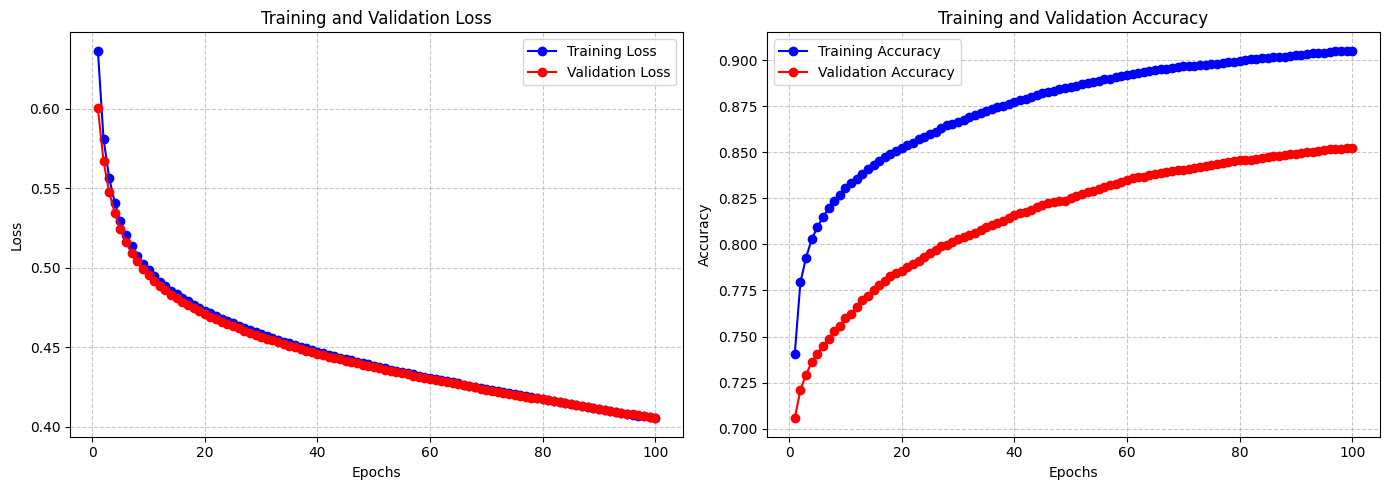
\includegraphics[width=0.7\linewidth]{images/task1-2}
	\caption{تغییرات دقت و هزینه در طی آموزش با مدل رگرسیون لجستیک}
	\label{fig:task1-1}
\end{figure}
\begin{lstlisting}
	Classification Report:
	precision        recall  f1-score   support
	
	Airplane         0.5455    0.3240    0.4065      1000
	Not Airplane     0.9281    0.9700    0.9486      9000
	
	accuracy                             0.9054     10000
	macro avg        0.7368    0.6470    0.6776     10000
	weighted avg     0.8899    0.9054    0.8944     10000
	
\end{lstlisting}

\begin{figure}[h]
	\centering
	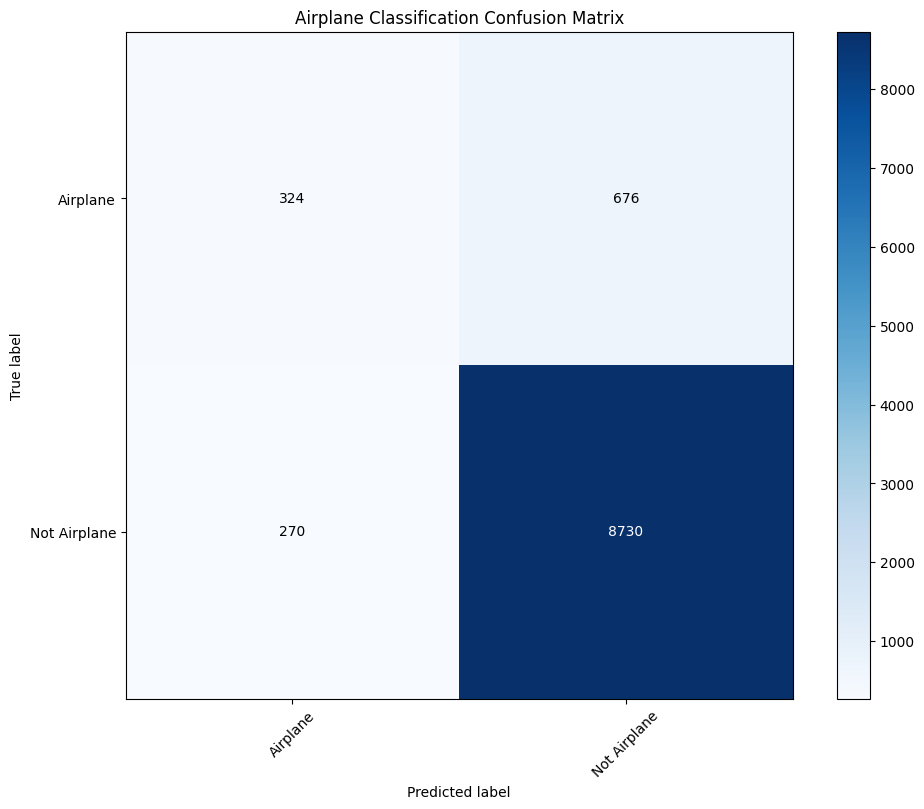
\includegraphics[width=0.5\linewidth]{images/task1-3}
	\caption{ماتریس آشفتگی برای مدل رگرسیون لاجستیک بعد ۱۰۰ ایپاک}
	\label{fig:task1-3}
\end{figure}


	\subsubsection{بخش دوم: شبکه با یک لایه پنهان}
	
	در این بخش، مدل با افزودن یک لایه پنهان با 64 نورون توسعه یافت. معماری شبکه به صورت زیر است:
	
	\[
	\begin{aligned}
		Z_1 &= W_1 X + b_1 \\
		A_1 &= \sigma(Z_1) \\
		Z_2 &= W_2 A_1 + b_2 \\
		A_2 &= \sigma(Z_2)
	\end{aligned}
	\]
	
	در اینجا نیز از سیگموئید به عنوان تابع فعال‌سازی استفاده شده و آموزش با الگوریتم گرادیان نزولی انجام شده است.
	
\begin{figure}[h]
	\centering
	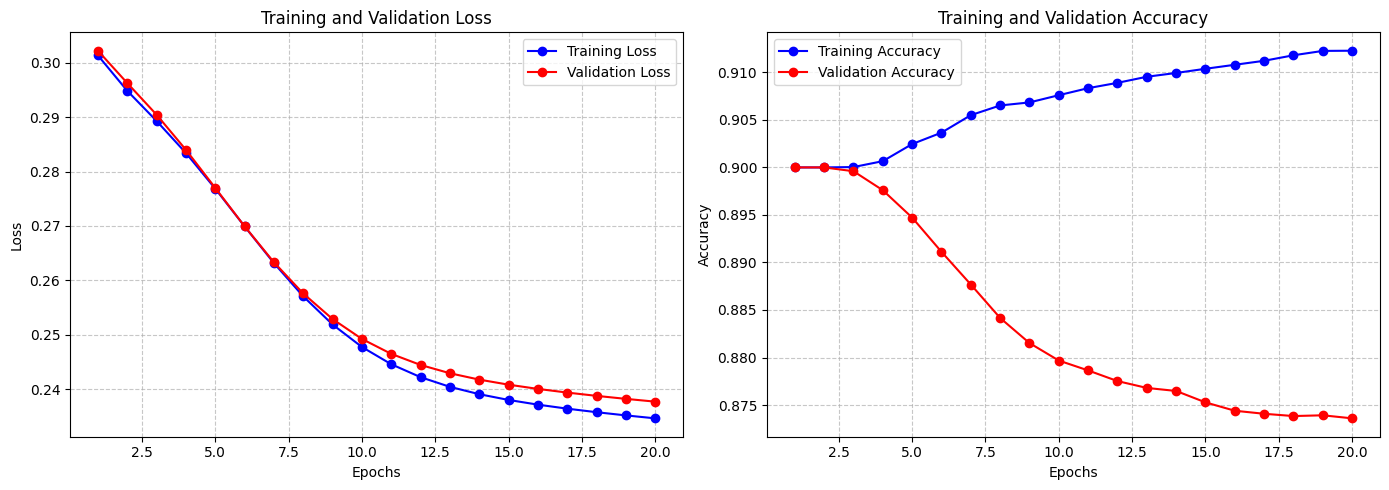
\includegraphics[width=0.7\linewidth]{images/task2-1}
	\caption{تغییرات دقت و هزینه در طی آموزش با مدل رگرسیون لجستیک چند لایه}
	\label{fig:task2-1}
\end{figure}


\begin{lstlisting}
	Classification Report:
	              precision    recall  f1-score   support
	
	Airplane         0.7000    0.2310    0.3474      1000
	Not Airplane     0.9205    0.9890    0.9535      9000
	
	accuracy                             0.9132     10000
	macro avg        0.8102    0.6100    0.6504     10000
	weighted avg     0.8984    0.9132    0.8929     10000
	
\end{lstlisting}

\begin{figure}[h]
	\centering
	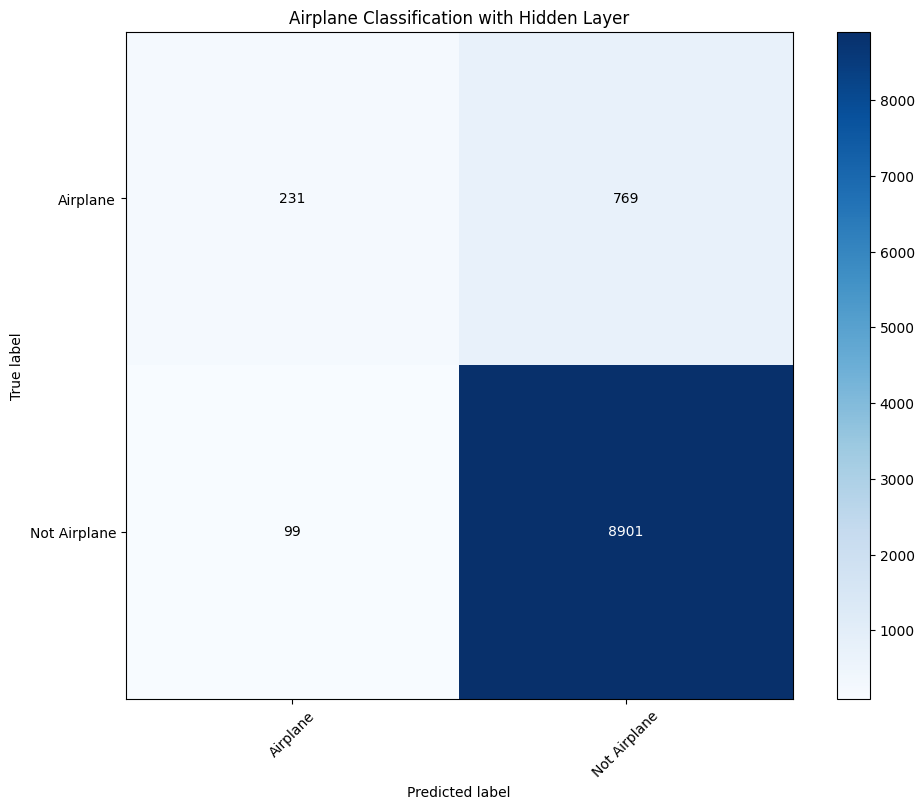
\includegraphics[width=0.5\linewidth]{images/task2-3}
	\caption{ماتریس آشفتگی برای مدل رگرسیون لاجستیک چند لایه بعد ۲۰ ایپاک}
	\label{fig:task1-3}
\end{figure}




	\subsubsection{بخش سوم: طبقه‌بندی چندکلاسه}
	
	در این مرحله، شبکه برای شناسایی تمامی ۱۰ کلاس \lr{CIFAR-10} طراحی شد. خروجی شبکه دارای ۱۰ نورون با تابع فعال‌سازی \lr{Softmax} است:
	
	\[
	\text{Softmax}(z_i) = \frac{e^{z_i}}{\sum_{j=1}^{10} e^{z_j}}
	\]
	
	تابع هزینه مورد استفاده، \lr{Categorical Cross-Entropy} است.
	
		
	\begin{figure}[h]
		\centering
		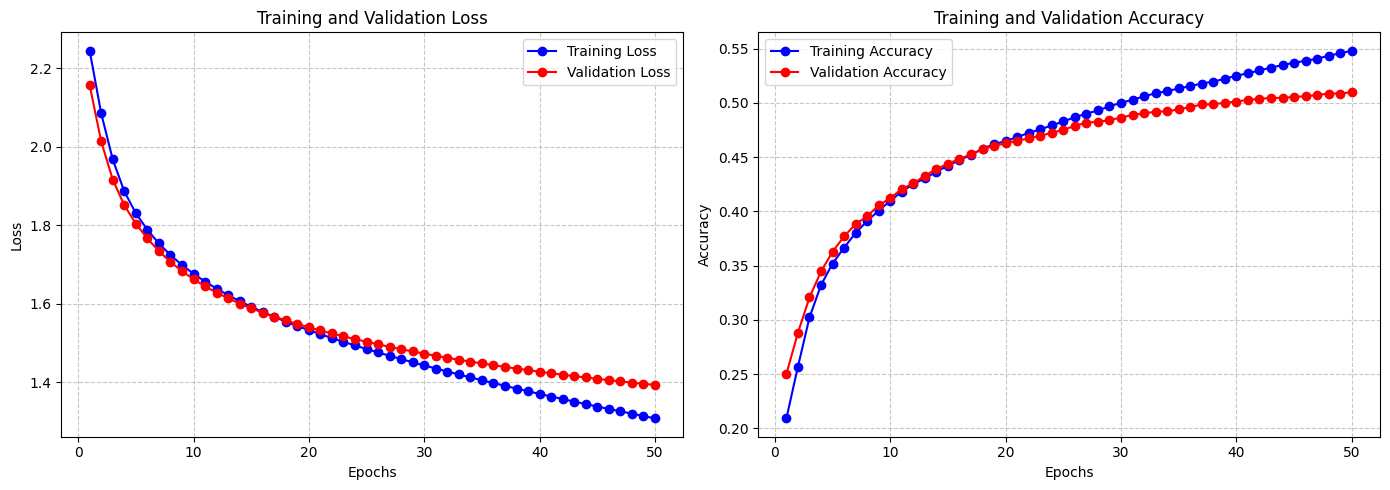
\includegraphics[width=0.7\linewidth]{images/task3-1}
		\caption{تغییرات دقت و هزینه در طی آموزش با مدل رگرسیون وان‌هات چند لایه}
		\label{fig:task3-1}
	\end{figure}
	
	
	
	\begin{lstlisting}
		Classification Report:
		precision                  recall  f1-score   support
		
		airplane         0.5959    0.5840    0.5899      1000
		automobile       0.6030    0.5970    0.6000      1000
		bird             0.4269    0.3270    0.3703      1000
		cat              0.3580    0.3430    0.3504      1000
		deer             0.4403    0.3800    0.4079      1000
		dog              0.4317    0.3920    0.4109      1000
		frog             0.4860    0.6400    0.5524      1000
		horse            0.5580    0.5720    0.5649      1000
		ship             0.5958    0.6750    0.6329      1000
		truck            0.5547    0.5880    0.5709      1000
		
		accuracy                             0.5098     10000
		macro avg        0.5050    0.5098    0.5051     10000
		weighted avg     0.5050    0.5098    0.5051     10000
		
	\end{lstlisting}
	
	\begin{figure}[h]
		\centering
		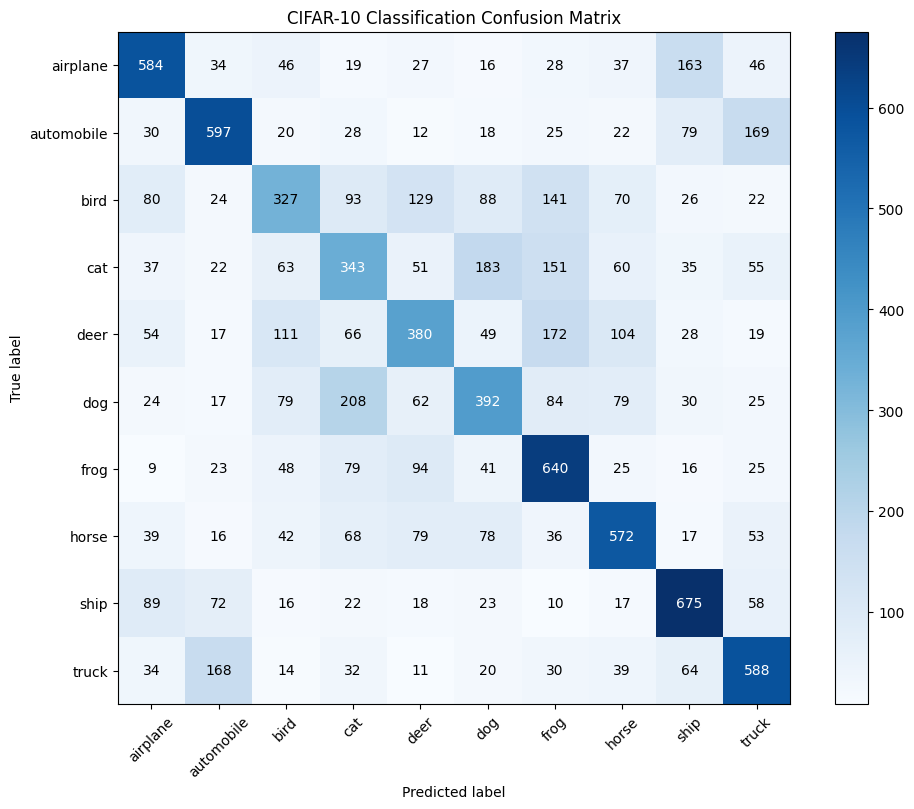
\includegraphics[width=0.8\linewidth]{images/task3-2}
		\caption{ماتریس آشفتگی برای مدل رگرسیون وان هات چند لایه بعد ۵۰ ایپاک}
		\label{fig:task3-2}
	\end{figure}
	
	
	
	
	
\subsubsection{بخش چهارم: مقایسه‌ی ویژگی‌های شبکه عصبی نیمه پیشرفته}
	
	در این بخش، یک شبکه عصبی نیمه پیشرفته با قابلیت استفاده از بهینه‌سازهای مختلف و توابع فعال‌سازی گوناگون پیاده‌سازی شده است. ساختار شبکه به‌گونه‌ای طراحی شده که از وزن‌دهی اولیه مناسب، ذخیره‌سازی گرادیان‌ها، و بهینه‌سازهای مدرن مانند Adam پشتیبانی می‌کند. 
	
	\subsubsection{توابع فعال‌سازی}
	
	توابع فعال‌سازی نقش مهمی در آموزش شبکه‌های عصبی ایفا می‌کنند. در این پروژه از سه تابع فعال‌سازی پرکاربرد شامل \lr{ReLU}، \lr{Sigmoid}، و \lr{Tanh} استفاده شده است.
	
	\begin{itemize}
		\item \textbf{تابع \lr{Sigmoid}:}
		\[
		\sigma(x) = \frac{1}{1 + e^{-x}}, \quad \sigma'(x) = \sigma(x)(1 - \sigma(x))
		\]
		
		\item \textbf{تابع \lr{Tanh}:}
		\[
		\tanh(x) = \frac{e^x - e^{-x}}{e^x + e^{-x}}, \quad \frac{d}{dx} \tanh(x) = 1 - \tanh^2(x)
		\]
		
		\item \textbf{تابع \lr{ReLU}:}
		\[
		f(x) = \max(0, x), \quad f'(x) = \begin{cases}
			1 & x > 0 \\
			0 & x \leq 0
		\end{cases}
		\]
	\end{itemize}

	
	در تحلیل تجربی، تابع ReLU به‌دلیل سادگی محاسباتی و اجتناب از مشکل ناپدید شدن گرادیان‌ها عملکرد برتری نسبت به سایر توابع نشان داد.
	
	\subsubsection{الگوریتم‌های بهینه‌سازی}
	
	در این پروژه سه الگوریتم زیر پیاده‌سازی و بررسی شده‌اند:
	\begin{enumerate}
		\item \lr{SGD}:
		به‌روزرسانی وزن‌ها به‌صورت مستقیم و بر پایه گرادیان فعلی صورت می‌گیرد:
		\[
		\theta = \theta - \eta \nabla_\theta J(\theta)
		\]
		که در آن \(\eta\) نرخ یادگیری و \(J(\theta)\) تابع هزینه است.
		
		\item \lr{Momentum}:
		این روش برای بهبود همگرایی، از سرعت قبلی استفاده می‌کند:
		\[
		v_t = \gamma v_{t-1} - \eta \nabla_\theta J(\theta) \quad,\quad \theta = \theta + v_t
		\]
		که در آن \(\gamma\) ضریب مومنتوم است.
		\item. \lr{Adam}:
		این روش تخمین‌هایی از میانگین و واریانس لحظه‌ای گرادیان‌ها ذخیره می‌کند:
		\[
		m_t = \beta_1 m_{t-1} + (1 - \beta_1) g_t
		\]
		\[
		v_t = \beta_2 v_{t-1} + (1 - \beta_2) g_t^2
		\]
		\[
		\hat{m}_t = \frac{m_t}{1 - \beta_1^t}, \quad \hat{v}_t = \frac{v_t}{1 - \beta_2^t}
		\]
		\[
		\theta = \theta - \eta \frac{\hat{m}_t}{\sqrt{\hat{v}_t} + \epsilon}
		\]
		\begin{figure}[h]
			\centering
			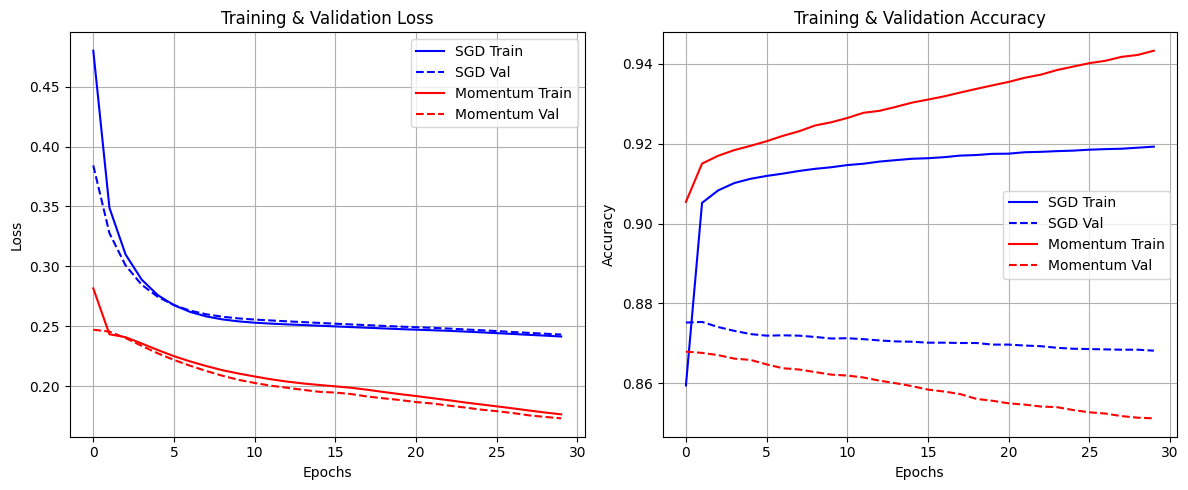
\includegraphics[width=0.7\linewidth]{images/task4-3}
			\caption{مقایسه‌ی همگرایی SGD و تکانه با فعال‌سازهای یکسان در دو لایه در داده‌های تست و آموزش}
			\label{fig:task4-3}
		\end{figure}
		
	
	\end{enumerate}
	

	
	
	
	\section*{مقداردهی اولیه وزن‌ها}
	
	برای بهبود عملکرد یادگیری، از دو روش مقداردهی اولیه استفاده شده است:
	
	\begin{itemize}
		\item \textbf{He Initialization} برای توابع ReLU:
		\[
		\text{Var}(w) = \frac{2}{n_{\text{in}}}
		\]
		
		\item \textbf{Xavier Initialization} برای توابع Sigmoid و Tanh:
		\[
		\text{Var}(w) = \frac{1}{n_{\text{in}}}
		\]
	\end{itemize}
	
	\begin{figure}[h]
		\centering
		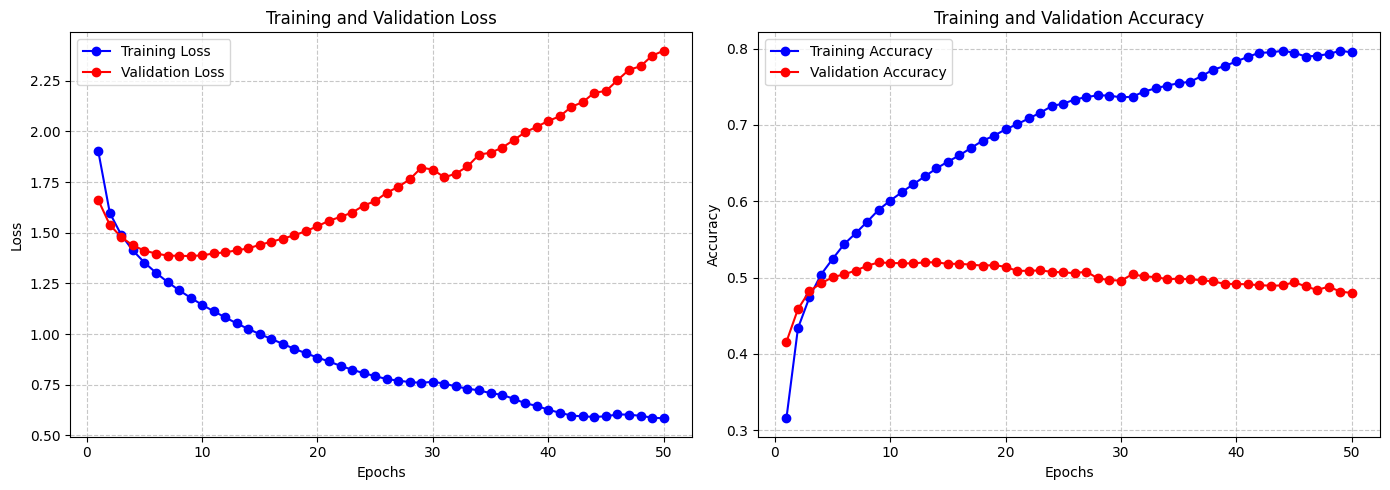
\includegraphics[width=0.7\linewidth]{images/task4-4}
		\caption{اثر مقداردهی اولیه He در یک شبکه دو لایه با بهینه‌ساز تکانه در ۳۰ ایپاک}
		\label{fig:task4-4}
	\end{figure}
	
	
	\section*{مقایسه تجربی توابع فعال‌سازی}
	
	در بخش سوم، برای مقایسه عملکرد توابع فعال‌سازی، سه شبکه با ساختار یکسان ولی با توابع ReLU، Sigmoid، و Tanh آموزش داده شد. نتایج نشان دادند که:
	
	\begin{itemize}
		\item ReLU منجر به همگرایی سریع‌تر و دقت بالاتر در داده‌های تست شد.
		\item Sigmoid به‌دلیل ناپدید شدن گرادیان در لایه‌های عمیق ضعیف‌ترین عملکرد را داشت.
		\item Tanh عملکردی بین دو تابع دیگر ارائه داد.
	\end{itemize}
		\begin{figure}[h]
		\centering
		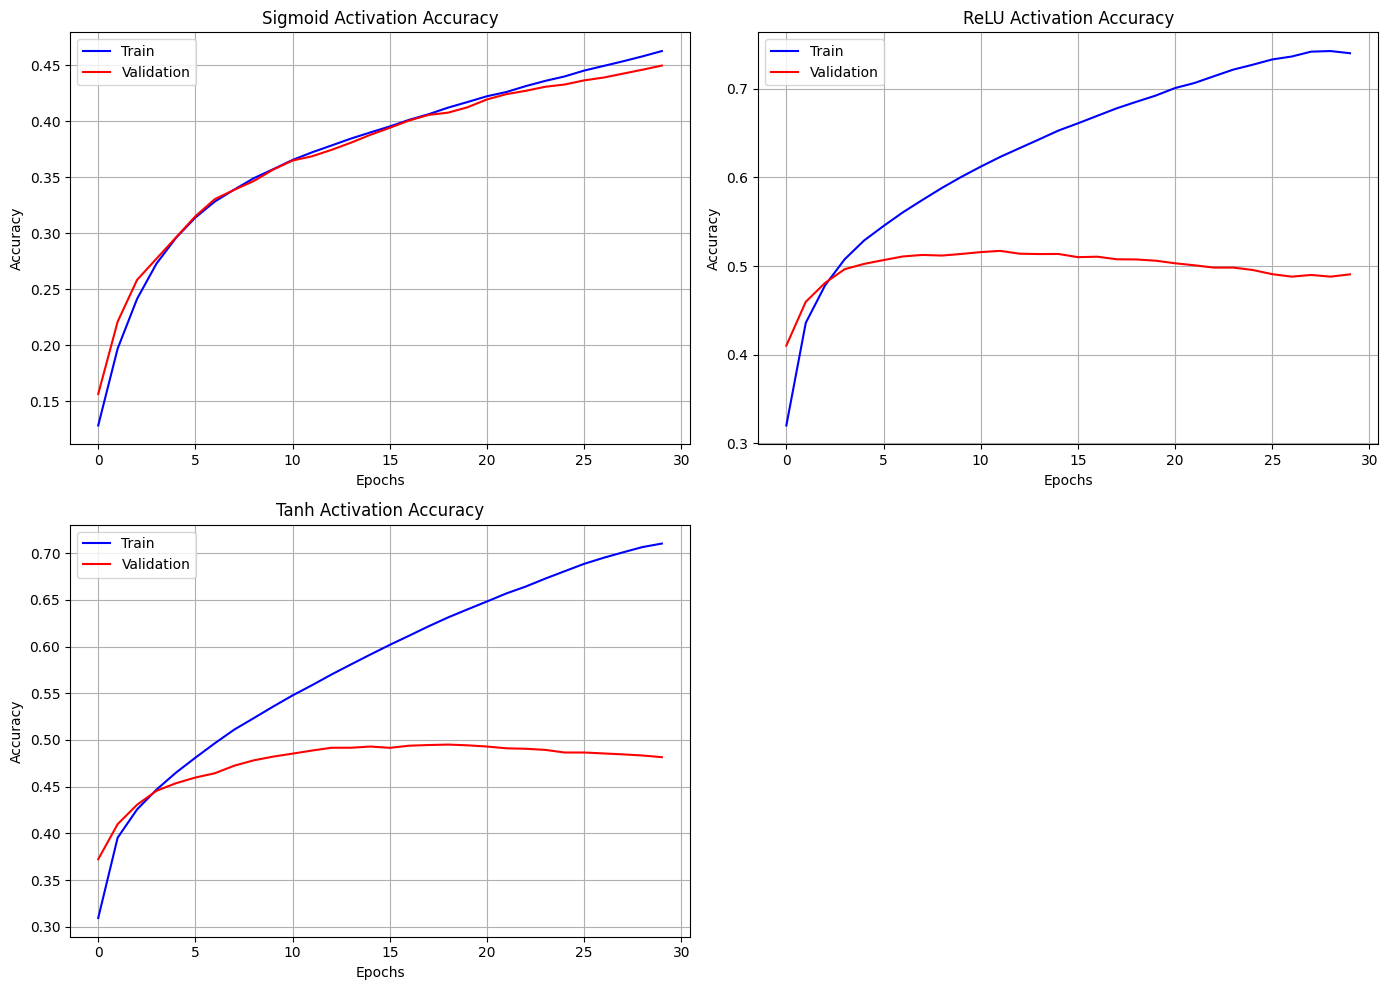
\includegraphics[width=0.7\linewidth]{images/task4-2}
		\caption{مقایسه‌ی همگرایی توابع فعالسازی متفاوت با ۳۰ ایپاک}
		\label{fig:task4-2}
	\end{figure}
	
	نتایج در قالب نمودارهای دقت در طول اپوک‌ها رسم گردیدند.
	
	\section*{مقایسه تجربی بهینه‌سازها}
	
	در بخش پایانی، عملکرد سه الگوریتم \lr{SGD}، \lr{Momentum} و \lr{Adam} بر روی یک شبکه سه‌لایه آزمایش شد. نتایج حاکی از آن بود که:
	
	\begin{itemize}
		\item Adam در اکثر موارد سریع‌تر همگرا شد و به دقت بالاتری رسید.
		\item Momentum پایداری بهتری نسبت به SGD داشت.
		\item استفاده از بهینه‌ساز مناسب نقش مهمی در کیفیت آموزش دارد.
	\end{itemize}
		
	\begin{figure}[h]
		\centering
		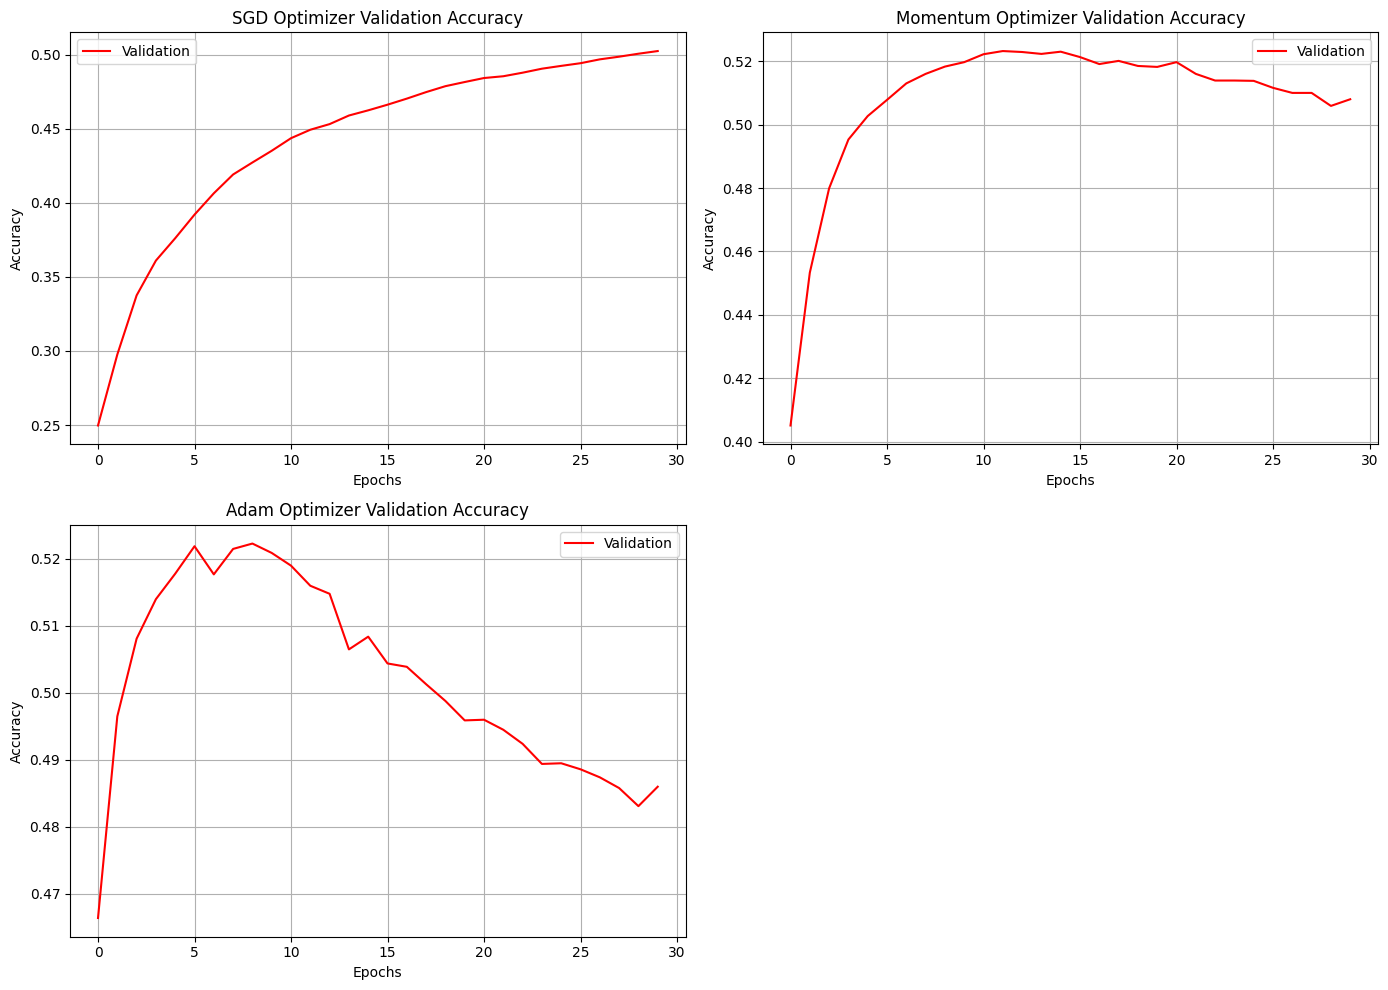
\includegraphics[width=0.7\linewidth]{images/task4-1}
		\caption{مقایسه‌ی همگرایی بین بهینه‌سازهای مختلف در ۳۰ ایپاک}
		\label{fig:task4-1}
	\end{figure}
	
	
	مدل طراحی‌شده در این پروژه به‌دلیل ساختار ماژولار و قابل گسترش، قابلیت استفاده در کاربردهای مختلف را دارد. نتایج تجربی نشان دادند که انتخاب دقیق تابع فعال‌سازی، مقداردهی اولیه مناسب، و الگوریتم بهینه‌سازی مؤثر نقش کلیدی در موفقیت مدل ایفا می‌کند.
	

\begin{enumerate}
	\item \textbf{گزارش پیاده‌سازی رگرسیون لجستیک برای طبقه‌بندی دودویی تصاویر CIFAR-10}
	
	\textbf{مقدمه}
	
	این گزارش به جزئیات پیاده‌سازی و ارزیابی یک مدل رگرسیون لجستیک از پایه در پایتون می‌پردازد. هدف اصلی، طبقه‌بندی دودویی تصاویر از مجموعه داده CIFAR-10 است، به این صورت که تشخیص دهد آیا تصویر "هواپیما" (کلاس 0) است یا "سایر کلاس‌ها". این پیاده‌سازی شامل مراحل بارگذاری داده، پیش‌پردازش، تعریف توابع فعال‌سازی و زیان، پیاده‌سازی مدل رگرسیون لجستیک با به‌روزرسانی گرادیان کاهشی و در نهایت ارزیابی عملکرد مدل است.
	
	\textbf{1. بارگذاری و نرمال‌سازی دیتاست CIFAR-10}
	
	مجموعه داده CIFAR-10 با استفاده از \texttt{torchvision.datasets.CIFAR10} بارگذاری شده است. تصاویر آموزشی و آزمون دانلود شده و سپس مقادیر پیکسل آن‌ها به بازه [0, 1] نرمال‌سازی شده‌اند با تقسیم بر 255.0. این مرحله تضمین می‌کند که مقادیر ورودی در یک مقیاس استاندارد قرار دارند، که برای فرآیند آموزش مدل‌های یادگیری ماشین ضروری است. علاوه بر این، میانگین تصاویر آموزشی از هر دو مجموعه داده آموزشی و آزمون کم شده است تا داده‌ها به سمت صفر مرکزی شوند (mean centering).
	
	\textbf{2. بازبرچسب‌گذاری داده‌ها}
	
	برای سناریوی طبقه‌بندی دودویی، برچسب‌های اصلی CIFAR-10 تغییر داده شده‌اند. اگر یک تصویر متعلق به کلاس "هواپیما" (برچسب 0) باشد، برچسب آن به 1 تغییر می‌کند؛ در غیر این صورت، برچسب آن به 0 تنظیم می‌شود. این تبدیل، مجموعه داده را برای طبقه‌بندی دودویی آماده می‌کند، جایی که 1 نشان‌دهنده کلاس مثبت (هواپیما) و 0 نشان‌دهنده کلاس منفی (سایر) است.
	
	\textbf{3. مسطح کردن (Flatten) تصاویر}
	
	تصاویر CIFAR-10 که در ابتدا دارای ابعاد (ارتفاع, عرض, کانال) هستند، به بردارهای یک‌بعدی مسطح شده‌اند. برای تصاویر CIFAR-10 که ابعاد آن‌ها 32x32 پیکسل با 3 کانال رنگی (RGB) است، هر تصویر به یک بردار با 3072 ویژگی (32 * 32 * 3) تبدیل می‌شود. این فرمت برای ورودی به مدل رگرسیون لجستیک مناسب است.
	
	\textbf{4. پیاده‌سازی توابع فعال‌سازی و زیان}
	
	\begin{itemize}
		\item \textbf{تابع فعال‌سازی سیگموئید ($\sigma(z)$)}: این تابع احتمال خروجی یک نورون در مدل رگرسیون لجستیک را محاسبه می‌کند. خروجی آن بین 0 و 1 قرار دارد. فرمول پیاده‌سازی شده:
		$$\sigma(z) = \frac{1}{1 + e^{-z}}$$
		
		\item \textbf{تابع زیان کراس-انتروپی دودویی (Binary Cross-Entropy Loss)}: این تابع زیان برای مسائل طبقه‌بندی دودویی استفاده می‌شود و میزان تفاوت بین توزیع احتمال پیش‌بینی شده و توزیع واقعی را اندازه‌گیری می‌کند. یک مقدار اپسیلون (1e-10) برای جلوگیری از لگاریتم صفر اضافه شده است. فرمول پیاده‌سازی شده:
		$$L(y_{true}, y_{pred}) = -\frac{1}{N} \sum_{i=1}^{N} [y_{true,i} \log(y_{pred,i}) + (1 - y_{true,i}) \log(1 - y_{pred,i})]$$
		
	\end{itemize}
	
	\textbf{5. پیاده‌سازی آموزش مدل با استفاده از گرادیان کاهشی}
	
	کلاس \texttt{LogisticRegression} یک مدل رگرسیون لجستیک را پیاده‌سازی می‌کند.
	
	\begin{itemize}
		\item \textbf{مقداردهی اولیه پارامترها}: وزن‌ها ($W$) با مقادیر تصادفی کوچک (ضربدر 0.01) و بایاس ($b$) با صفر مقداردهی اولیه می‌شوند.
		\item \textbf{پیش‌بینی احتمالات (predict\_probabilities)}: این متد با استفاده از فرمول رگرسیون لجستیک، احتمالات خروجی را محاسبه می‌کند: $z = XW + b$ و $a = \sigma(z)$.
		\item \textbf{محاسبه گرادیان‌ها (compute\_gradients)}: گرادیان‌های مربوط به وزن‌ها ($dW$) و بایاس ($db$) با استفاده از فرمول‌های گرادیان برای کراس-انتروپی دودویی محاسبه می‌شوند:
		
		
		$dz = y_{pred} - y_{true}$
		
		
		$dW = \frac{1}{m} X^T dz$
		
		
		$db = \frac{1}{m} \sum dz$
		
		که در آن $m$ تعداد نمونه‌ها در بچ است.
		\item \textbf{به‌روزرسانی پارامترها (update\_params)}: وزن‌ها و بایاس با استفاده از نرخ یادگیری ($lr$) و گرادیان‌های محاسبه شده به‌روزرسانی می‌شوند:
		$W \leftarrow W - lr \cdot dW$
		
		
		$b \leftarrow b - lr \cdot db$
		
		\item \textbf{آموزش (train)}: متد \texttt{train} مدل را برای تعداد مشخصی از اپوک‌ها بر روی داده‌های آموزشی آموزش می‌دهد. این متد بر روی دسته‌های کوچک داده (mini-batches) تکرار می‌کند، احتمالات را پیش‌بینی می‌کند، زیان را محاسبه می‌کند، گرادیان‌ها را محاسبه کرده و پارامترها را به‌روزرسانی می‌کند. میانگین زیان و دقت هر اپوک را نیز ذخیره می‌کند.
		\item \textbf{پیش‌بینی (predict)}: این متد بر اساس آستانه 0.5، پیش‌بینی‌های دودویی (0 یا 1) را انجام می‌دهد.
	\end{itemize}
	
	برای دسته‌بندی داده‌ها به صورت دسته‌ای، یک کلاس \texttt{SimpleLoader} پیاده‌سازی شده است که قابلیت دسته‌بندی و ترکیب تصادفی (shuffling) داده‌ها را فراهم می‌کند.
	
	\textbf{6. ارزیابی مدل}
	
	مدل پس از آموزش با استفاده از معیارهای \texttt{confusion\_matrix} و \texttt{f1\_score} بر روی مجموعه داده آزمون ارزیابی شد. همچنین یک تابع \texttt{classification\_report} برای نمایش دقیق‌تر معیارهای \texttt{precision}, \texttt{recall} و \texttt{f1-score} برای هر کلاس استفاده شده است.
	
	برای یافتن بهترین آستانه طبقه‌بندی (threshold) که عملکرد مدل را به حداکثر می‌رساند، یک جستجو در بازه \lr{[0.1, 0.9]} با 17 نقطه (intervals) انجام شد. بهترین آستانه بر اساس بالاترین امتیاز F1-score انتخاب گردید.
	
	\textbf{نتایج ارزیابی:}
	
	پس از 200 اپوک با نرخ یادگیری \lr{0.0001} و اندازه بچ 512:
	
	\begin{itemize}
		\item \textbf{بهترین آستانه}: \lr{0.50}
		\item \textbf{بهترین F1-score}: \lr{0.4460}
		\item \textbf{دقت آزمون (\lr{Test Accuracy})}: \lr{0.8872}
	\end{itemize}
	
	\textbf{ماتریس درهم‌ریختگی (\lr{Confusion Matrix}):}
	
	\begin{tabular}{|l|l|l|}
		\hline
		& Pred Other & Pred Airplane \\ \hline
		True Other    & 8418       & 582           \\ \hline
		True Airplane & 546        & 454           \\ \hline
	\end{tabular}
	
	
	\textbf{گزارش طبقه‌بندی (\lr{Classification Report}):}
	
	\begin{tabular}{|l|l|l|l|l|}
		\hline
		& precision & recall & f1-score & support \\ \hline
		Other        & \lr{0.9391}    & \lr{0.9353} & \lr{0.9372 }  & \lr{9000}    \\ \hline
		Airplane     & \lr{0.4382}    & \lr{0.4540} &\lr{ 0.4460}   & \lr{1000}    \\ \hline
		\textbf{accuracy} &           &        & \textbf{\lr{0.8872}} & \lr{10000}   \\ \hline
		macro avg    & \lr{0.6887 }   & \lr{0.6947} & \lr{0.6916}   & \lr{10000}   \\ \hline
		weighted avg & \lr{0.8890}    & \lr{0.8872} &\lr{ 0.8881}   & \lr{10000}   \\ \hline
	\end{tabular}
	
	
	\textbf{تحلیل نتایج:}
	
	دقت کلی مدل \lr{ 0.8872} است که نشان‌دهنده عملکرد نسبتاً خوب مدل در طبقه‌بندی صحیح تصاویر است. با این حال، با بررسی \texttt{classification\_report}، مشخص می‌شود که عملکرد مدل برای کلاس "Other" (سایر) بسیار بهتر از کلاس "Airplane" (هواپیما) است.
	
	\begin{itemize}
		\item \textbf{کلاس "Other"}: دارای precision، recall و F1-score بالایی است (حدود \lr{0.93}). این نشان می‌دهد که مدل در شناسایی تصاویر "سایر" هم دقیق است (تعداد کمی از "هواپیما"ها را به اشتباه "سایر" دسته‌بندی می‌کند) و هم پوشش خوبی دارد (اکثر تصاویر "سایر" را به درستی شناسایی می‌کند).
		\item \textbf{کلاس "Airplane"}: دارای precision، recall و F1-score به مراتب پایین‌تری است (حدود \lr{0.44}). این نشان می‌دهد که مدل در شناسایی تصاویر "هواپیما" دقت و پوشش کمتری دارد. به عبارت دیگر، تعداد قابل توجهی از تصاویر "هواپیما" به اشتباه به عنوان "سایر" دسته‌بندی شده‌اند (recall پایین) و از بین تصاویری که مدل به عنوان "هواپیما" پیش‌بینی کرده، تعداد زیادی در واقع "سایر" بوده‌اند (precision پایین).
	\end{itemize}
	
	\textbf{چالش‌ها و بهبودهای احتمالی:}
	
	عملکرد ضعیف برای کلاس "هواپیما" می‌تواند ناشی از عدم توازن داده‌ها باشد؛ تعداد نمونه‌های کلاس "هواپیما" (1000) بسیار کمتر از کلاس "سایر" (9000) است.
	
	\textbf{نمودارهای زیان و دقت آموزش:}
	
	نمودارها نشان‌دهنده کاهش پیوسته زیان آموزش و افزایش دقت آموزش در طول اپوک‌ها هستند، که حاکی از یادگیری مدل است. نمودار ها در داخل کد دیده می شوند.
	
	
	\textbf{نتیجه:}
	
	مدل رگرسیون لجستیک به خوبی برای طبقه‌بندی دودویی تصاویر CIFAR-10 پیاده‌سازی و آموزش داده شد. با وجود دقت کلی مناسب، مدل در شناسایی کلاس اقلیت ("هواپیما") چالش‌هایی دارد. این موضوع می‌تواند در بخش‌های بعدی با استفاده از شبکه‌های عمیق‌تر و راهکارهای مدیریت عدم توازن داده‌ها بهبود یابد.
		
	\item بخش 2
	\item بخش3
	\item بخش 4
	\item بخش 5
\end{enumerate}
